\documentclass{article}

% Environment setup

\usepackage[
    margin=.75in
]{geometry} %geometry (sets margin) and other useful packages 

\setlength{\parindent}{0em}
\setlength{\parskip}{.5em}

\usepackage{graphicx}
\usepackage{grffile}  % support extra dots in filenames
\usepackage{fancyref}
\usepackage[labelfont=bf]{caption}
\usepackage{subcaption}

\usepackage{chngcntr} \counterwithin{figure}{section} \counterwithin{table}{section}


\title{\textbf{CS 4641:} Markov Decision Processes}
\author{Bradley Reardon}
\date{April 14, 2019}

\begin{document}
  \maketitle

  \section{Introduction}
    In this paper, we will be exploring the use of Markov Decision Processes and Reinforcement Learning to model and find optimal solutions for specific problem spaces. For the purpose of analysis, this report will cover applying various algorithms to two problems, which are completing a level of a classic Block Dude game, and navigating through a grid world. In exploring Markov Decision Processes, we will evaluate both problems using both value iteration and policy iteration. Afterward, we will explore each algorithm further, by applying Reinforcement Learning to the algorithms using Q-Learning.

  \section{Grid World}

    \subsection{Domain}
      We will begin by discussing the Grid World problem. In the context of a Markov Decision Process, this problem space is relatively small. For each given position on the grid, there are a maximum of only 4 possible actions, which are movements to the north, south, east, and west. In addition, the goal is fixed and only requires movement actions to transitition to the goal state. Lastly, the grid's wall positions are fixed and do not change as a result of any transition.

      Because of the properties of this problem space specifically, the Grid World problem can be hypothesized to converge to an optimal solution relatively quickly. \Fref{fig:gw-domain} shows the three grid world ``levels'' that will be tested for the grid world domain.

      \begin{figure}[htb]
      \centering

        \begin{subfigure}{0.3\textwidth}
          \frame{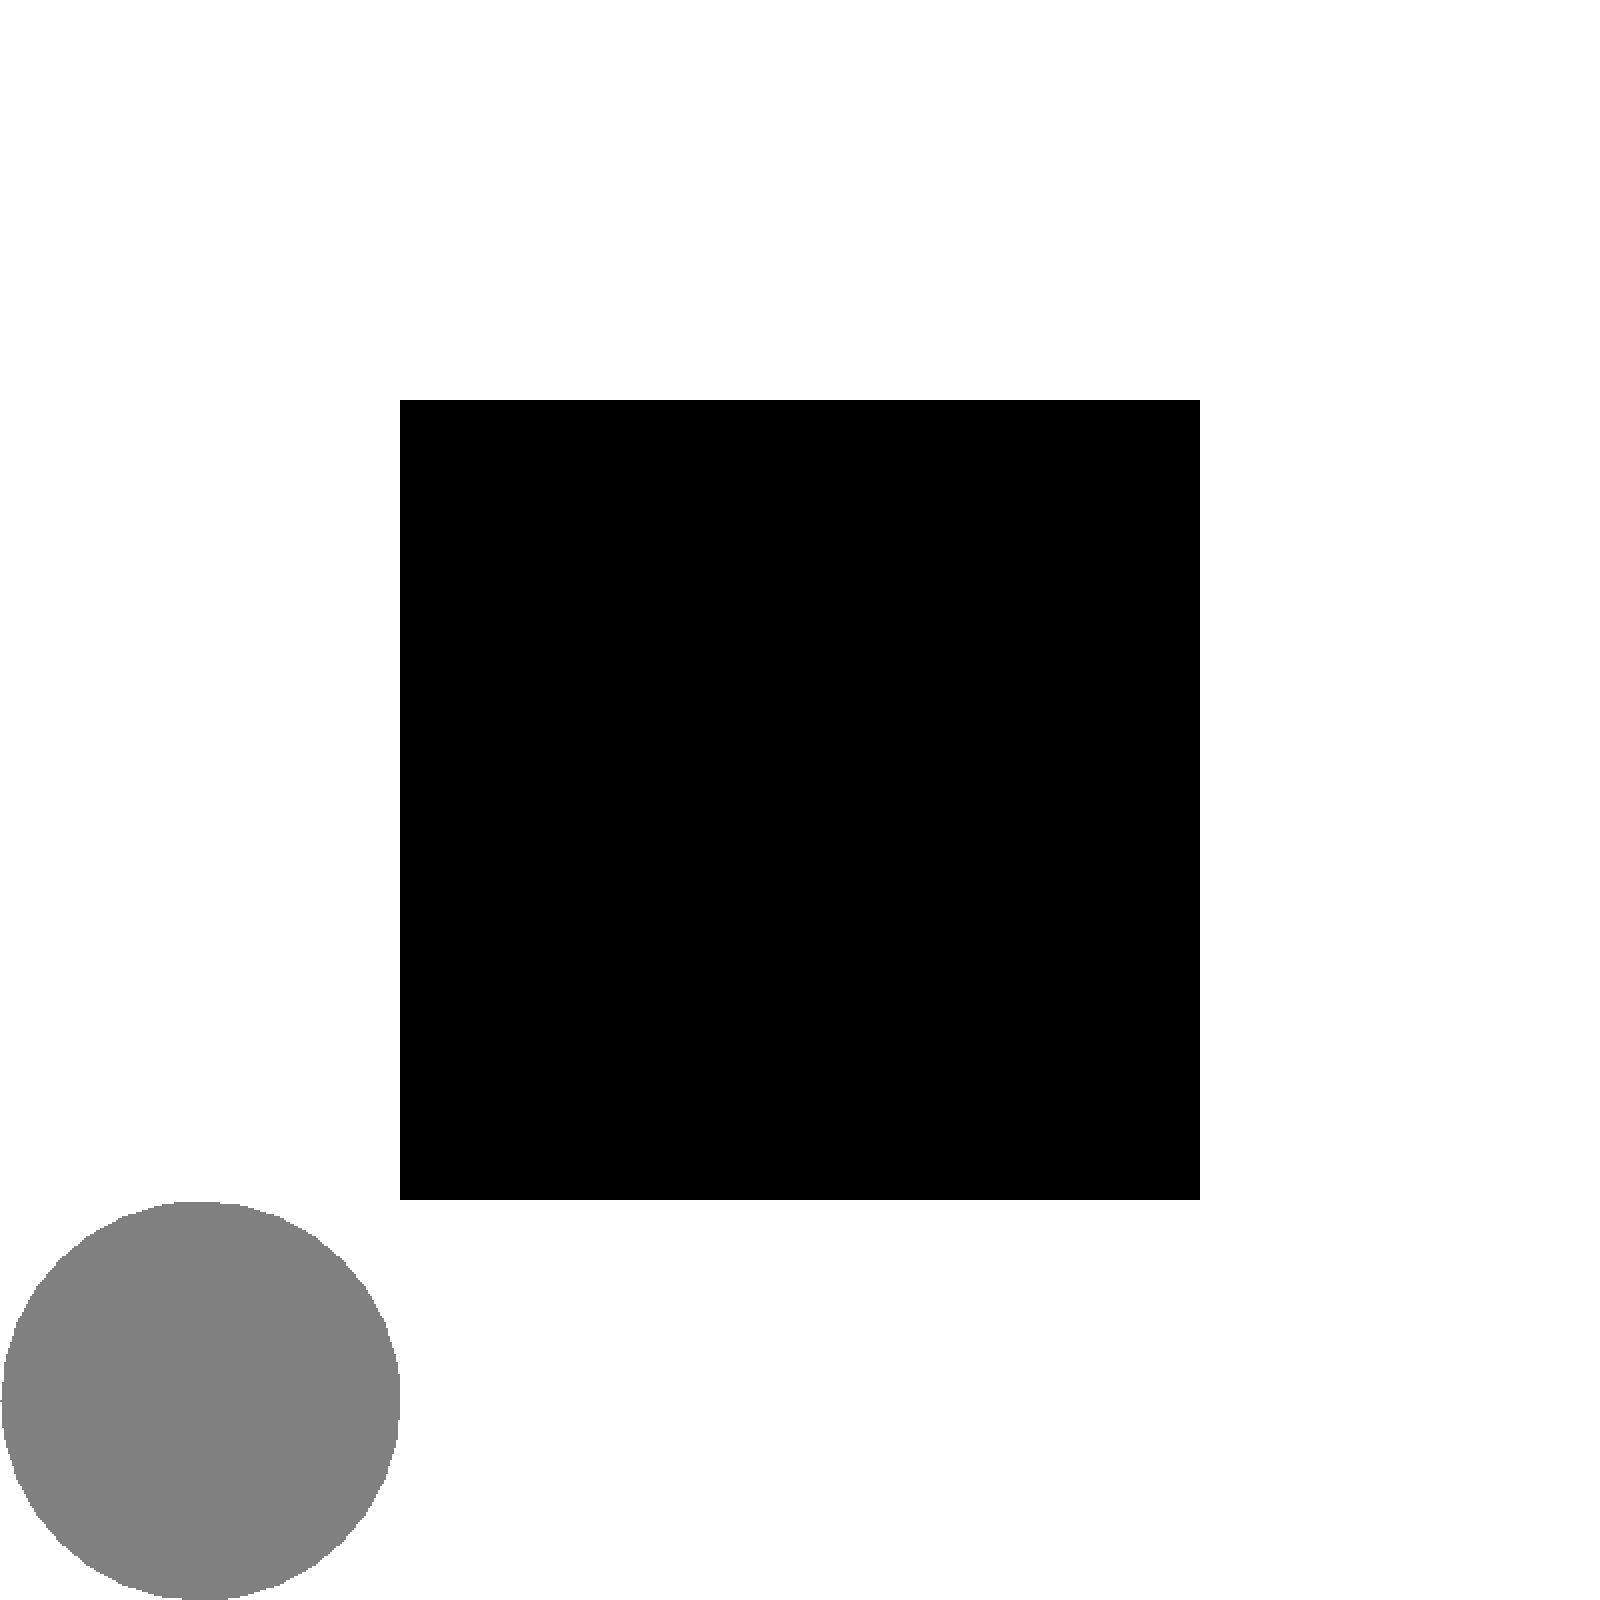
\includegraphics[width=\linewidth]{fig/gw-block}}
          \caption{Level 1: Single block}
        \end{subfigure}\hfil
        \begin{subfigure}{0.3\textwidth}
          \frame{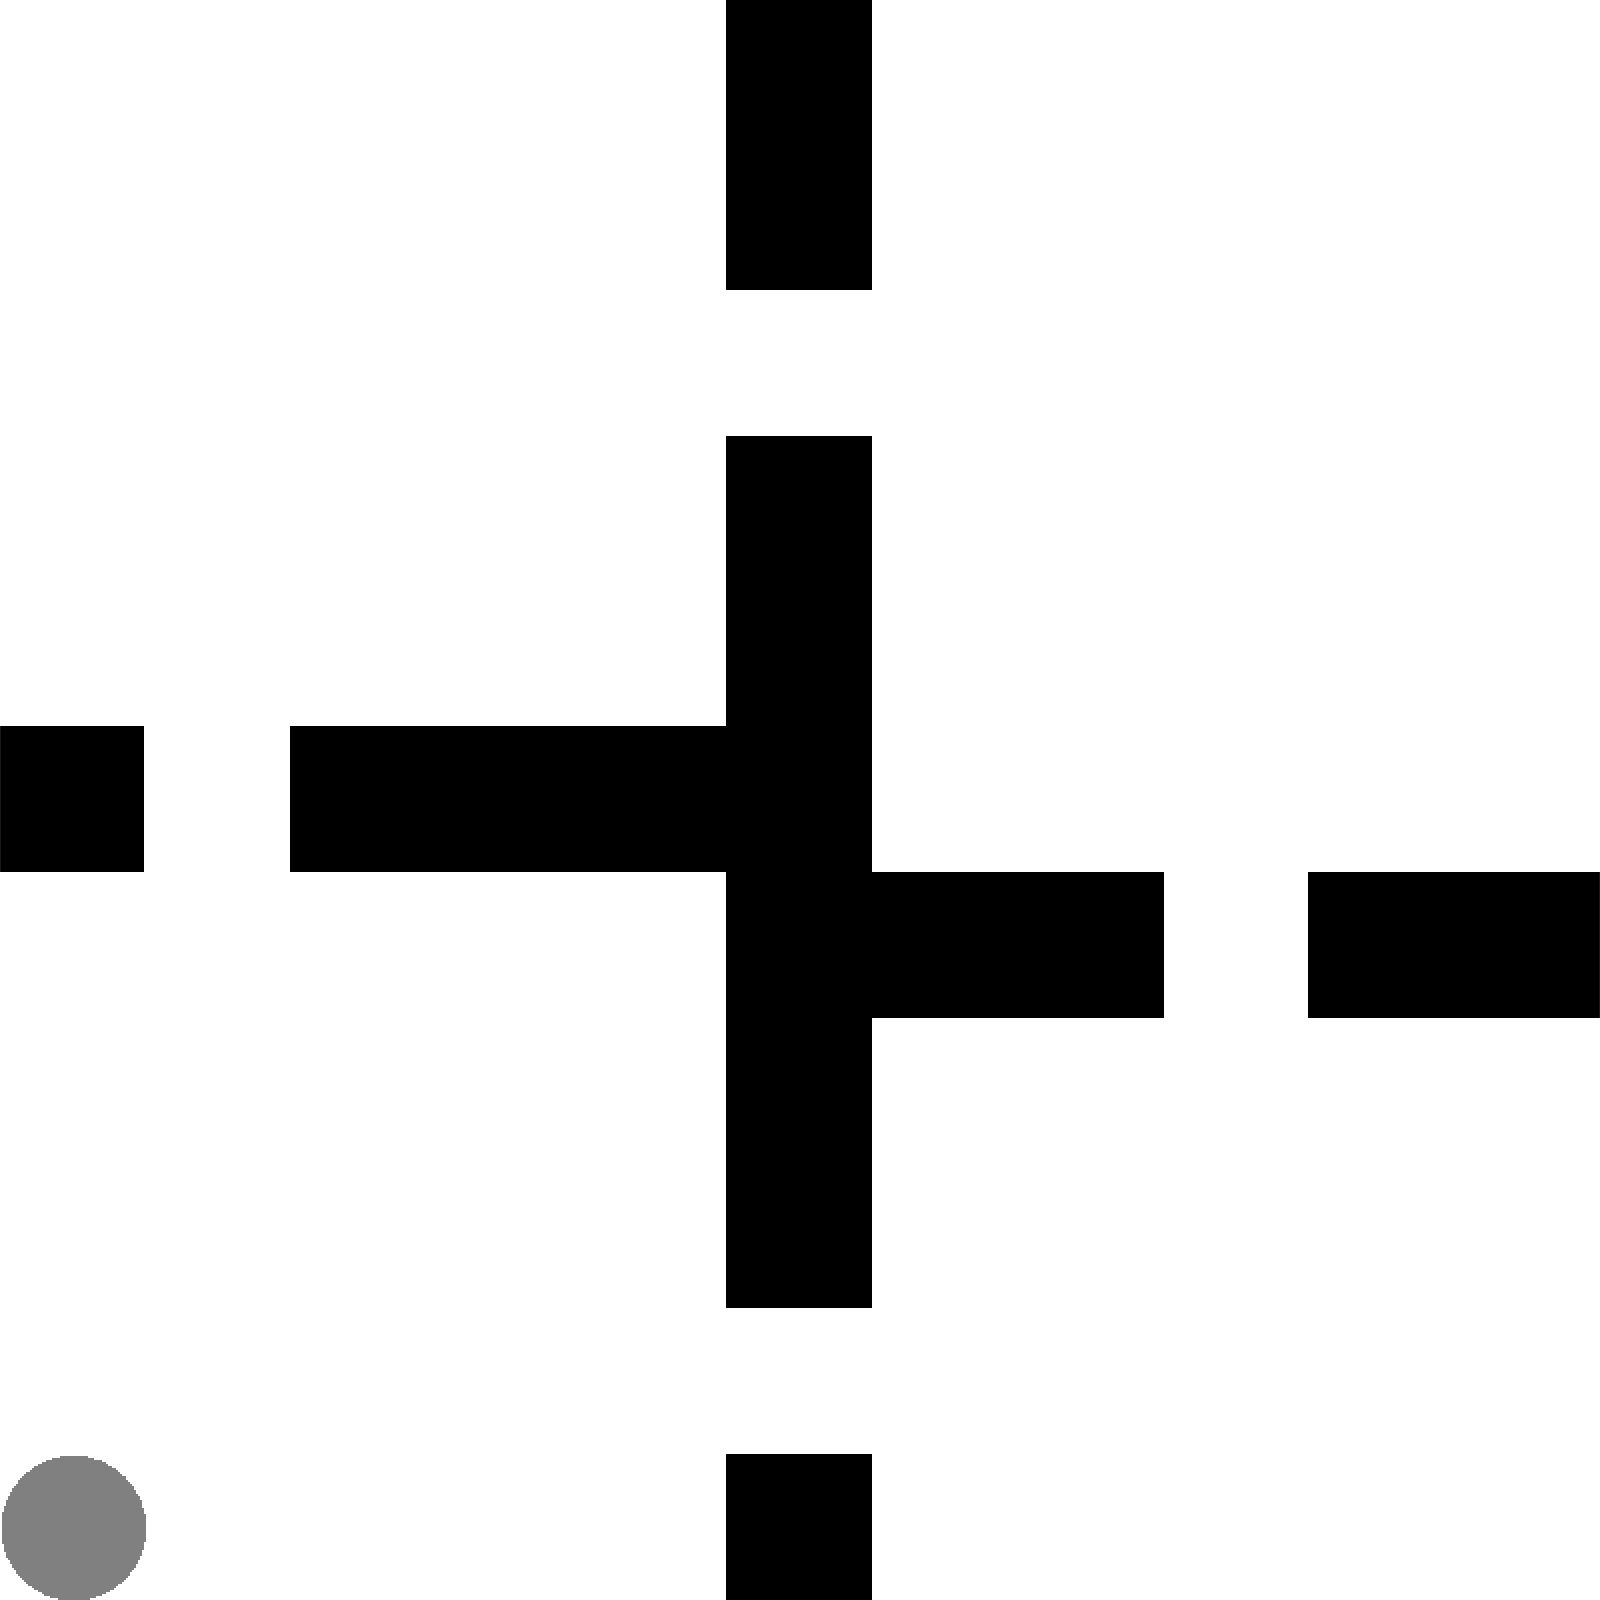
\includegraphics[width=\linewidth]{fig/gw-rooms}}
          \caption{Level 2: Four rooms}
        \end{subfigure}\hfil
        \begin{subfigure}{0.3\textwidth}
          \frame{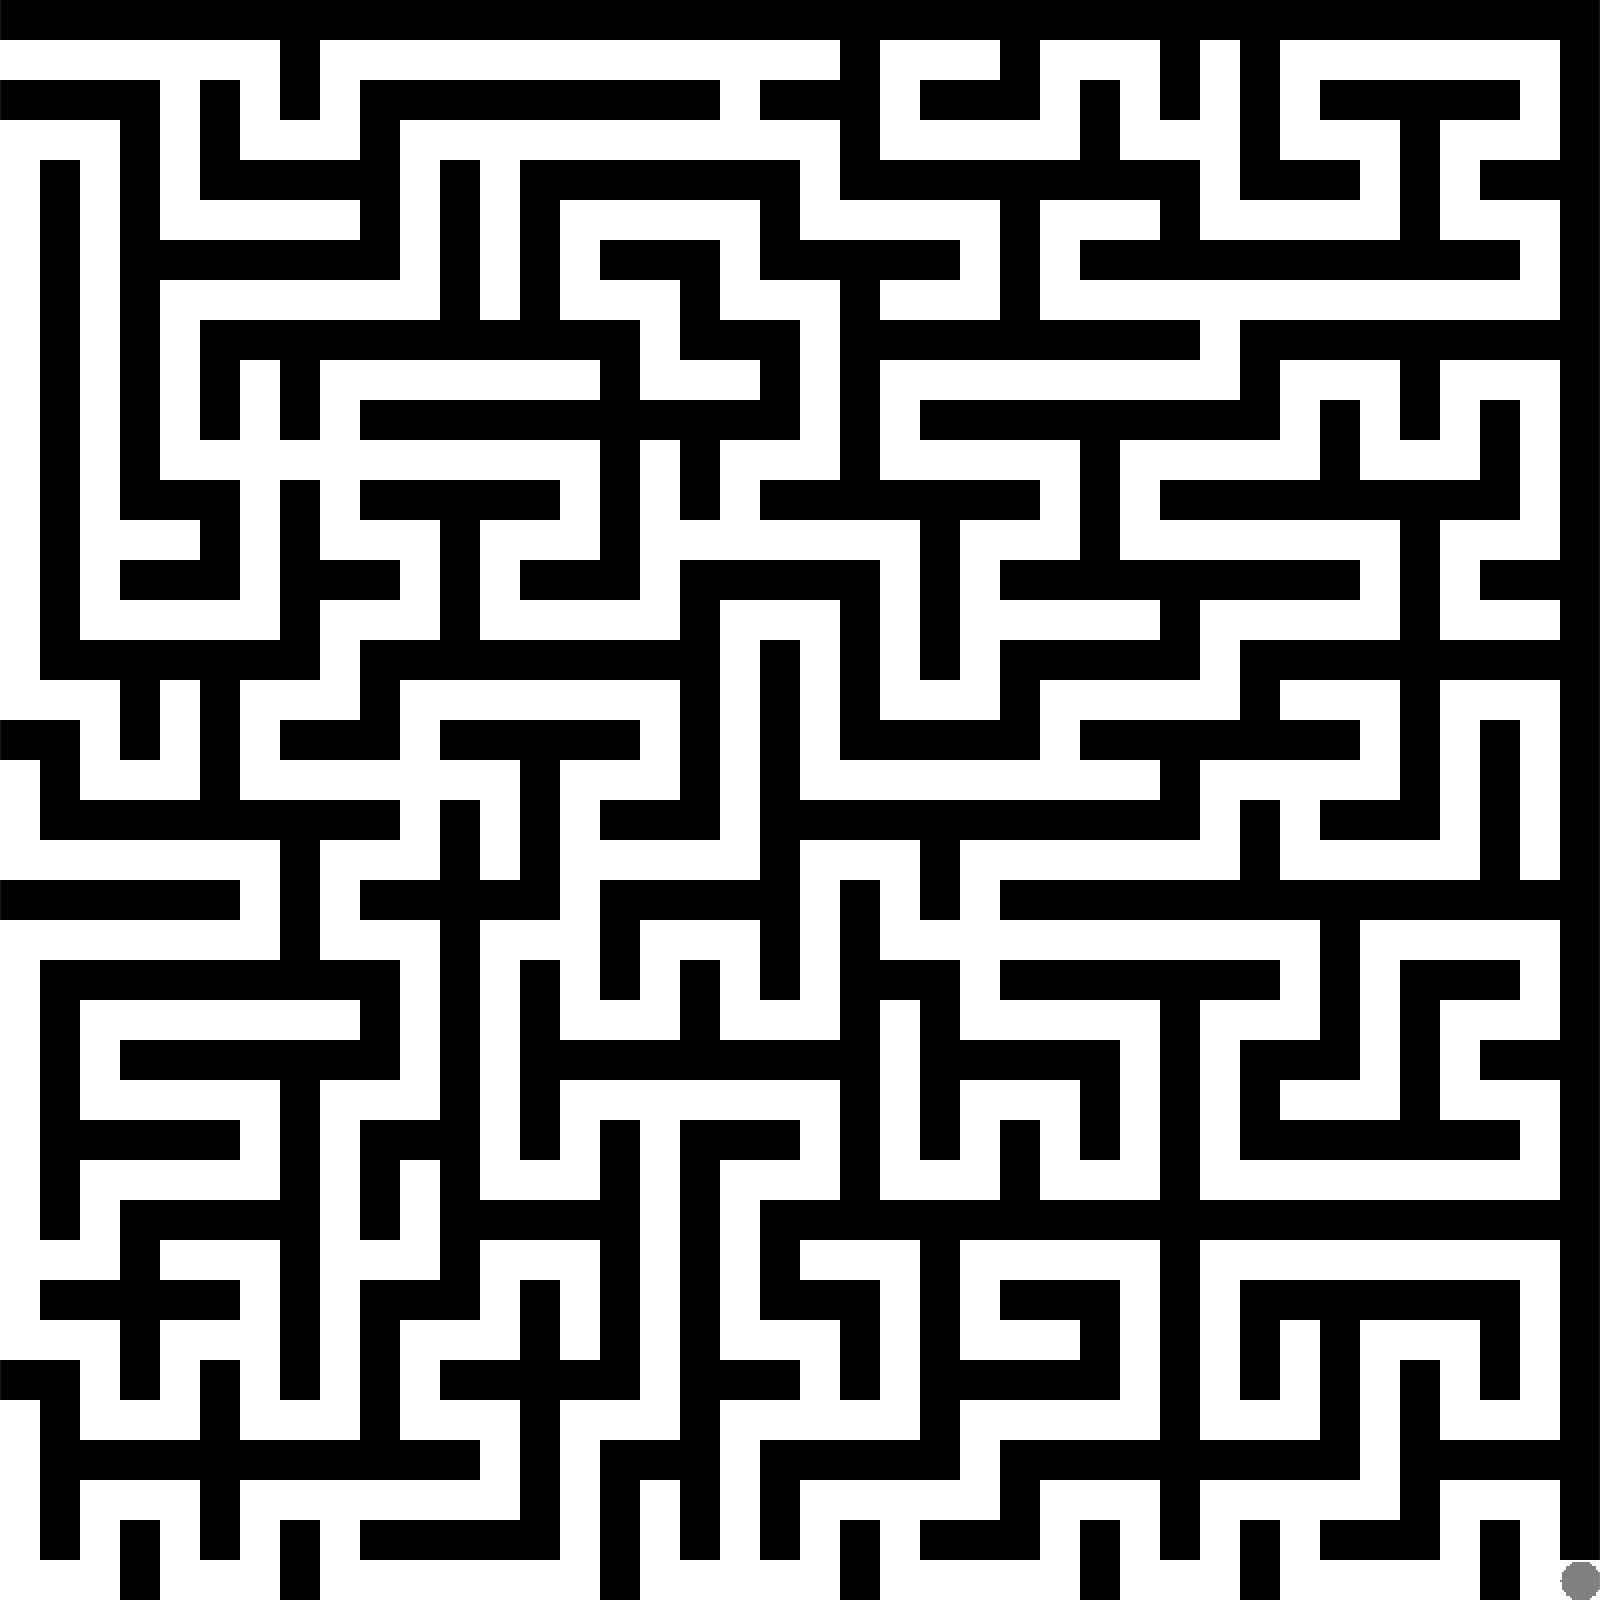
\includegraphics[width=\linewidth]{fig/gw-maze}}
          \caption{Level 3: Maze}
        \end{subfigure}

      \caption{Grid World levels}
      \label{fig:gw-domain}
      \end{figure}

      This problem is particularly interesting due to its relationship to path-finding. Since we're evaluating the best way to go through a known world, this problem has connections to robotics and artificial intelligence.

    \subsection{Value Iteration}
      Each of the three levels in the grid world experiment were tested using value iteration. Value iteration was run with a termination reward of 5.0, a step reward of -0.1, and a discount of 0.99. \Fref{tab:gw-vi-results} shows the statistics collected for each level.

      \begin{table}[h]
      \centering
        \begin{tabular}{|l|l|l|l|} \hline
          & \textbf{L1: Single Block} & \textbf{L2: Four Rooms} & \textbf{L3: Maze} \\ \hline
          \textbf{States} & 12 & 104 & 800 \\ \hline
          \textbf{Iterations} & 11 & 23 & 188 \\ \hline
          \textbf{Steps Taken} & 7 & 29 & 212 \\ \hline
          \textbf{Runtime} & 33ms & 123ms & 1.451s \\ \hline
        \end{tabular}

      \caption{Grid World: Value iteration results}
      \label{tab:gw-vi-results}
      \end{table}

    \subsection{Policy Iteration}
      After being run with value iteration, the experiment was run again using policy iteration. Policy iteration was run with the same parameters as value iteration, with a termination reward of 5.0, a step reward of -0.1, and a discount of 0.99. These values were chosen to evaluate consistency across the two algorithms, and to see which algorithm performs better under the same conditions. \Fref{tab:gw-pi-results} shows the results for this run.

      \begin{table}[h]
      \centering

        \begin{tabular}{|l|l|l|l|} \hline
          & \textbf{L1: Single Block} & \textbf{L2: Four Rooms} & \textbf{L3: Maze} \\ \hline
          \textbf{States} & 12 & 104 & 800 \\ \hline
          \textbf{Iterations} & 4 & 7 & 15 \\ \hline
          \textbf{Steps Taken} & 8 & 22 & 204 \\ \hline
          \textbf{Runtime} & 185ms & 696ms & 11.066s \\ \hline
        \end{tabular}

      \caption{Grid World: Policy iteration results}
      \label{tab:gw-pi-results}
      \end{table}

    \subsection{Q-Learning}
      \Fref{tab:gw-ql-results} shows the results for running Q-Learning on all three levels. In this case, the chosen learning rate was 0.1, the chosen qInit was 100, and episilon was 0.1. All three world models were trained over 2500 episodes. Interestingly, the maze world failed to complete the experiment and would stall when attempting to plan a path using the model. As such, these results will be denoted ``DNF''.

      \begin{table}[h]
      \centering

        \begin{tabular}{|l|l|l|l|} \hline
          & \textbf{L1: Single Block} & \textbf{L2: Four Rooms} & \textbf{L3: Maze} \\ \hline
          \textbf{Steps Taken} & 6 & 25 & DNF \\ \hline
          \textbf{Runtime} & 178ms & 426ms & DNF \\ \hline
        \end{tabular}

      \caption{Grid World: Q-Learning results}
      \label{tab:gw-ql-results}
      \end{table}

    \subsection{Discussion}
      Interestingly, these results suggest that value iteration is much faster on average at higher degrees of state complexity than policy iteration. However, most noticably, the maze level has a more optimial solution when policy iteration is used (204 steps) as opposed to value iteration (212 steps). Though the solution is marginally better for the maze world in the case of policy iteration, the 7.62-times increase in the runtime for the same world appears not to be worth the marginal improvement in solution optimization. This note will be revisited after experimenting with the Block Dude problem.

      As for Q-Learning, it outperformed policy iteration for levels 1 and 2, though it did fail to complete for the maze level. In the case of level 1, the solution contained the fewest steps yet, while in the case of level 2, the solution only outperformed that of value iteration. Overall, however, reinforcement learning via Q-Learning seems to be a reasonable choice for finding quick solutions to the Grid World problem, as long as the state space isn't too large. However, as a larger state space indicates larger complexity overall, and my computer has performance bottlenecks due to its age, it is impossible for me to make a determination as to whether Q-Learning is a good choice for runs on larger state spaces such as the Grid World maze.

  \section{Block Dude}

    \subsection{Domain}
      Next, we will evaluate the Block Dude game in the context of a Markov Decision Process. In this world, the ``block dude'' character has the ability to move around east, west, and up. In addition, gray blocks in the world are able to be picked up and placed down again in other locations. The addition of changing the world, in addition to the interest in the path-finding nature of the Grid World problem, makes the Block Dude game more complex than Grid World.

      In this section, we will be evaluating the same algorithms in two different Block Dude levels, which can be seen in \Fref{fig:bd-domain}.

      \begin{figure}[htb]
      \centering

        \begin{subfigure}{0.45\textwidth}
          \frame{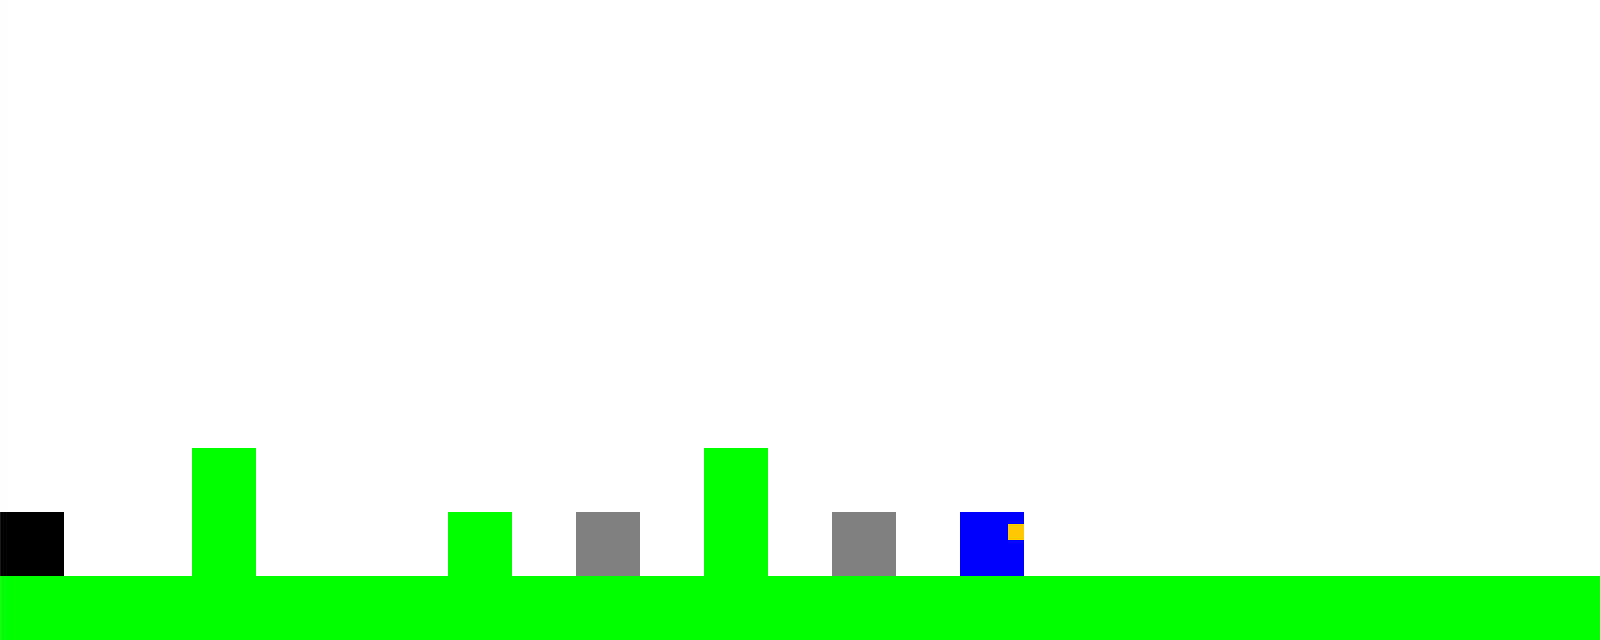
\includegraphics[width=\linewidth]{fig/bd-level1}}
          \caption{Level 1: Easy}
        \end{subfigure}\hfil
        \begin{subfigure}{0.45\textwidth}
          \frame{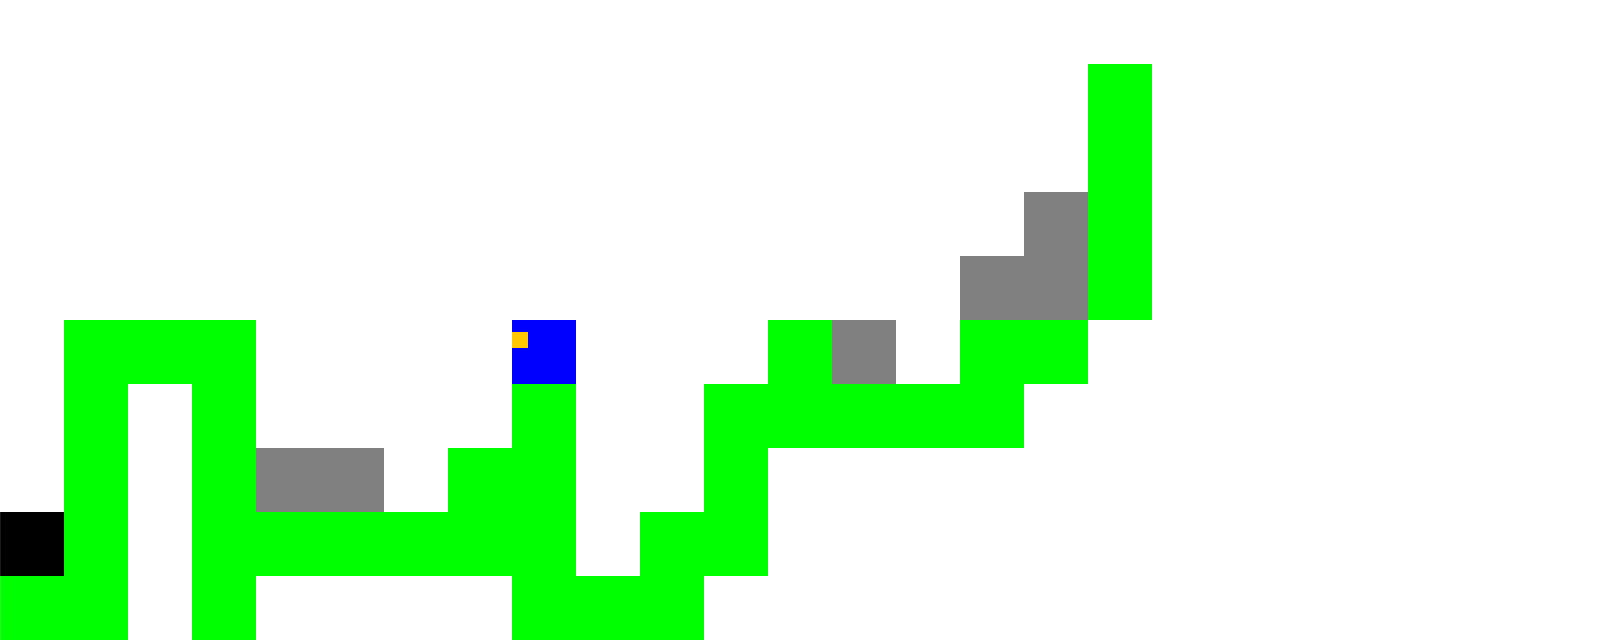
\includegraphics[width=\linewidth]{fig/bd-level2}}
          \caption{Level 2: Hard}
        \end{subfigure}\hfil

      \caption{Block Dude levels}
      \label{fig:bd-domain}
      \end{figure}

      As demonstrated by both levels, the nature of this game requires that the player change the terrain in order to reach the goal, making this a very interesting problem to explore in this context.

    \subsection{Value Iteration}
      \Fref{tab:bd-vi-results} shows the results for running value iteration on the easy and hard levels of Block Dude. It is instantly apparent based on the overall number of states that even the easy level of Block Dude exceeds the maze level of Grid World in terms of overall complexity. Value iteration in this case was again run with a termination reward of 5.0, a step reward of -0.1, and a discount of 0.99.

      \begin{table}[h]
      \centering
        \begin{tabular}{|l|l|l|} \hline
          & \textbf{L1: Easy} & \textbf{L2: Hard} \\ \hline
          \textbf{States} & 841 & 14200 \\ \hline
          \textbf{Iterations} & 230 & 230 \\ \hline
          \textbf{Steps Taken} & 19 & 94 \\ \hline
          \textbf{Runtime} & 4.016s & 66.637s \\ \hline
        \end{tabular}

      \caption{Block Dude: Value iteration results}
      \label{tab:bd-vi-results}
      \end{table}

    \subsection{Policy Iteration}
      Next, policy iteration was run. The overall choice in parameters was again the same to keep consistent results in evaluating policy iteration versus value iteration. \Fref{tab:bd-pi-results} shows the results for this test.

      \begin{table}[h]
      \centering
        \begin{tabular}{|l|l|l|} \hline
          & \textbf{L1: Easy} & \textbf{L2: Hard} \\ \hline
          \textbf{States} & 840 & 14199 \\ \hline
          \textbf{Iterations} & 20 & 52 \\ \hline
          \textbf{Steps Taken} & 19 & 94 \\ \hline
          \textbf{Runtime} & 13.076s & 940.171s \\ \hline
        \end{tabular}

      \caption{Block Dude: Policy iteration results}
      \label{tab:bd-pi-results}
      \end{table}

    \subsection{Q-Learning}
      Unfortunately, for the Block Dude problem, a similar problem to the one above from the Grid World maze level was encountered during Q-Learning. As a result, no result was obtainable from either the easy or hard levels of the Block Dude problem.

    \subsection{Discussion}
      In the end, the results show that the Block Dude is a very single-approach game in terms of the required steps to arrive at a solution. In both successful tests using value and policy iteration respectively, both algorithms resulted in equally-optimal solutions for each level. However, the main difference between the two approaches is that per-iteration runtime is much higher in the case of policy iteration, so much so that the hard level required nearly 16 minutes to reach a solution. In this case, value iteration stands out as the clear winner in terms of overall performance, as nothing is gained from the major performance hit from taking a policy-iterative approach in solving the level.

  \section{Discussion}
    For the two problems explored in this report, value iteration was the clear-winning approach in all cases. Though in some tests policy iteration or Q-Learning resulted in solutions that took fewer steps (mainly in the case of Grid World), the performance tradeoffs of switching to a different approach in the context of these problems was not worth it.

    However, this isn't to discredit the efficacy of the policy iteration and Q-Learning algorithms. Policy iteration takes many fewer iterations to converge to a solution on average than value iteration itself, suggesting that for some problems with much larger complexity spaces that policy learning may have an advantage in converging faster over time. However, this was not the case in any of our tests.

    For Q-Learning, though three of the five tests failed to complete with the testing implementation used for this project, the reinforcement learning algorithm did show similar results to the other algorithms on two of the Grid World tests. With further parameter tuning and a better understanding of the implementation of this algorithm in BURLAP, this may have been able to be avoided. However, with the constraint of time, this was not able to be explored further.

  \section{Conclusion}
    In closing, I have attempted to evaluate Markov Decision Processes and Reinforcement Learning in the context of two interesting problems. Value iteration and policy iteration, despite their simple approach, proved effective in all cases explored in this report, though the performance tradeoffs of using policy iteration in this case are a point of further discussion.

    Future explorations of this topic may lead to an attempt to iteratively optimize the parameters of each of these methods for learning, however the parameters used throughout the various sections of the report did prove sufficient for experimentation. 


\end{document}